\section{Database Annotation Errors} \label{sec:Clustering_Anomalies}

\begin{table}[!hbt]
    \centering
    \caption[Anomalies in Segment 4 Cluster 2 (\Acrshort{PCA})]{\textbf{Anomalies in Segment 4 Cluster 2 (\Acrshort{PCA}).}.}
    \label{tab:PCA_Error_4_2}
    \pgfplotstabletypeset[
        every head row/.style={
            before row={
                \toprule
            },
            after row={
                \midrule
            },
        },
        every last row/.style={
            after row={
                %... & ... & ... & ... & ... & ... & ... & ...\\
                \bottomrule
            },
        },
        begin table=\begin{tabular*}{0.75\textwidth},
        end table=\end{tabular*},
        columns={0,1,2},
        columns/0/.style={string type,multicolumn names=l,column name=\textbf{Accession}, column type=@{\extracolsep{\fill}\hspace{6pt}}r},
        columns/1/.style={multicolumn names=l,column name=\textbf{H1}, column type=r},
        columns/2/.style={multicolumn names=l,column name=\textbf{H10}, column type=r},
    ]
    {PCA/error_segment_4_cluster_2_difference_head.csv}
\end{table}

\begin{table}[!hbt]
    \centering
    \caption[Anomalies in Segment 4 Cluster 48 (\Acrshort{PCA})]{\textbf{Anomalies in Segment 4 Cluster 48 (\Acrshort{PCA}).}.}
    \label{tab:PCA_Error_4_48}
    \pgfplotstabletypeset[
        every head row/.style={
            before row={
                \toprule
            },
            after row={
                \midrule
            },
        },
        every last row/.style={
            after row={
                ... & ... & ...\\
                \bottomrule
            },
        },
        begin table=\begin{tabular*}{0.75\textwidth},
        end table=\end{tabular*},
        columns={0,1,2},
        columns/0/.style={string type,multicolumn names=l,column name=\textbf{Accession}, column type=@{\extracolsep{\fill}\hspace{6pt}}r},
        columns/1/.style={multicolumn names=l,column name=\textbf{H16}, column type=r},
        columns/2/.style={multicolumn names=l,column name=\textbf{H13}, column type=r},
    ]
    {PCA/error_segment_4_cluster_48_difference_head.csv}
\end{table}

\begin{figure}[!hbt]
    \centering
    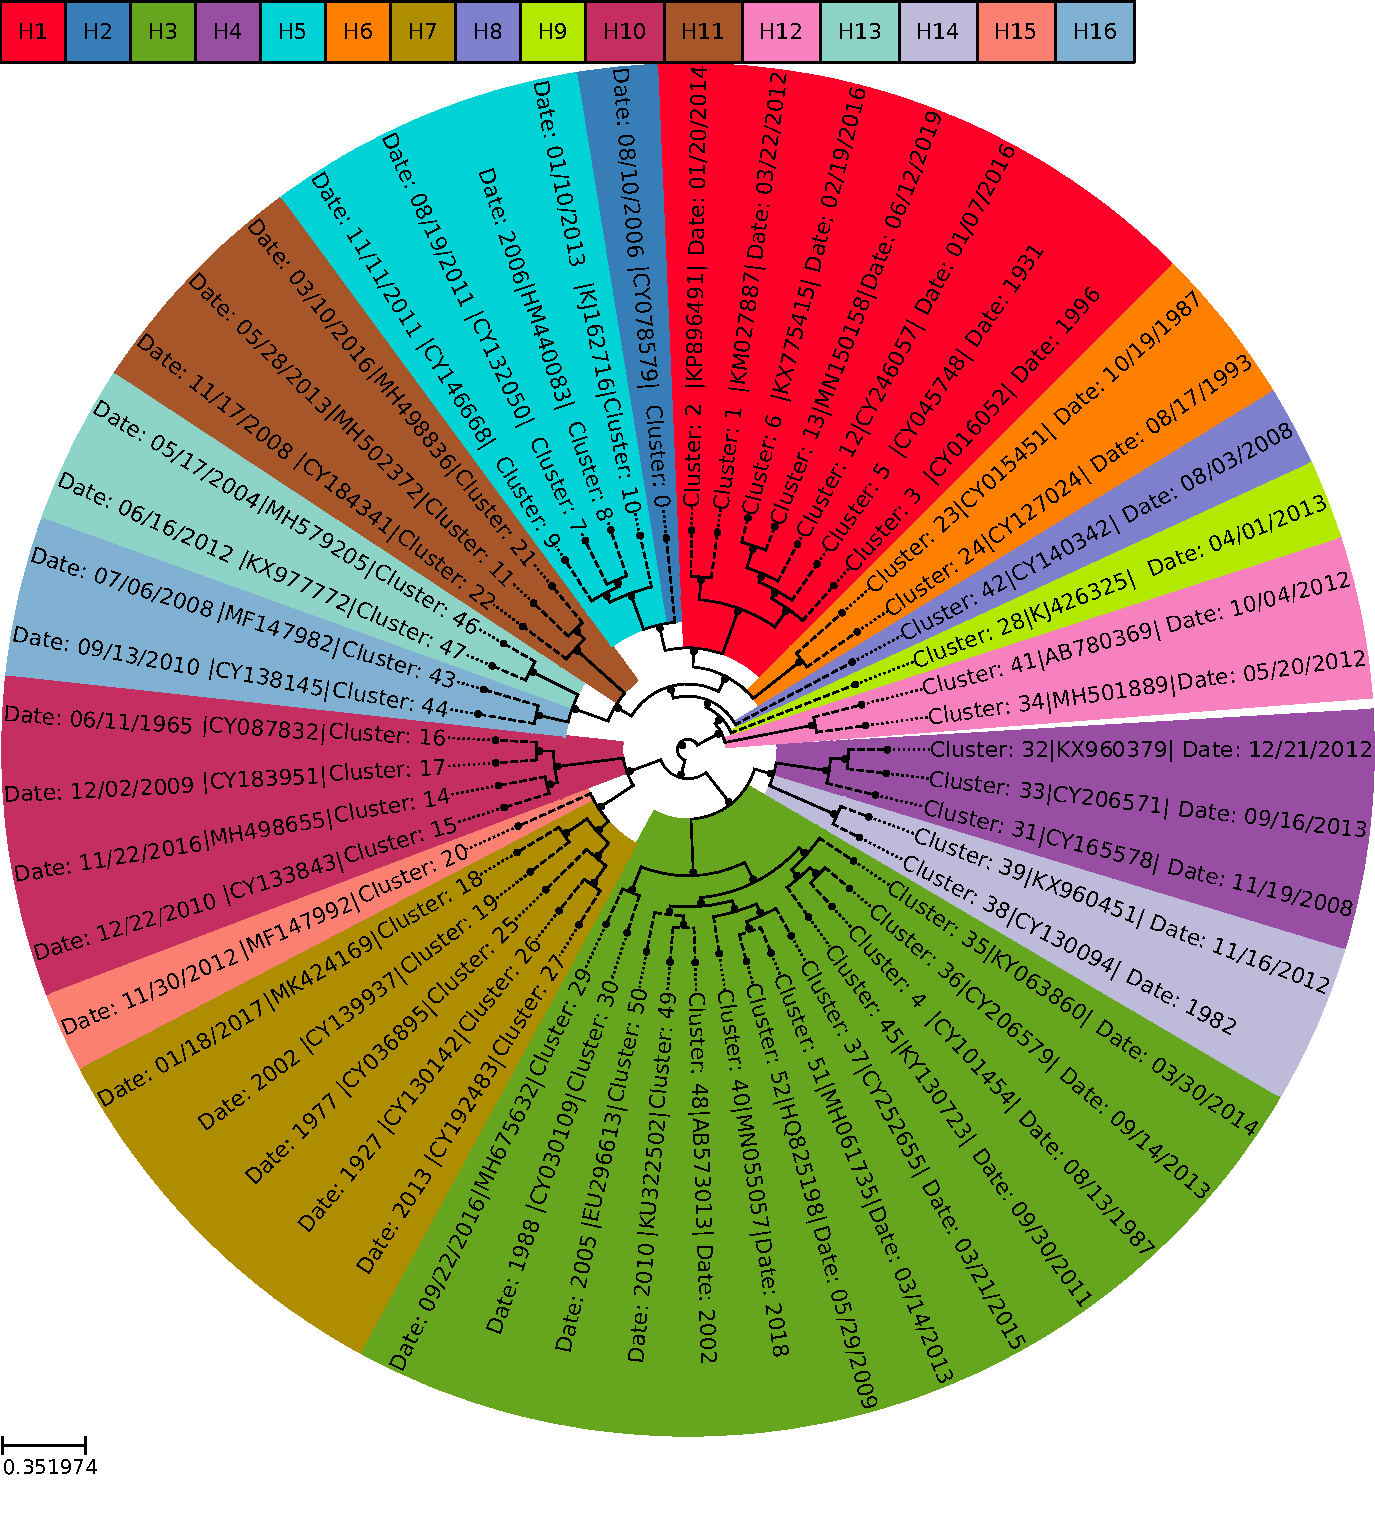
\includegraphics[width=\textwidth]{PCA/Guidetree_segment_4_H_Centroid.pdf}
    \caption[Knee based Segment 4 Centroid Guidetree (\Acrshort{PCA})]{\textbf{Knee based Segment 4 Centroid Guidetree (\Acrshort{PCA}).} .}
    \label{fig:PCA_Guidetree_Centroid_4}
\end{figure}

%Übergang zu cluster Comparison durch Centroid Alignment Tree -> H13/H16 Clustertree, Alignmenttree Vergleich -> Cluster H13/H16 Comparison
%fehler im clustering oder fehler in der DAtenbank